\section{Code Quality}\label{sec:code_quality}
The term code quality defines an evaluation of source code concerning the readability and understandability the source code. If source code is well-written and can be understood by developers easily, it is considered to be high quality.

One of the main reasons why companies and developers aim for high code quality is the maintainability of source code. With a better understandability of the source code, changing it becomes more efficient and less error-prone.
Software maintenance consists mainly of those activities that involve changing source code:
\begin{enumerate}
    \item Adding code for new features
    \item Implementing changing requirements by modifying code
    \item Fixing bugs to ensure correct functionality of the software.
\end{enumerate}
The importance of good maintainability of source code is based on the associated cost.
For project planning, different sources suggest planning 50 to 80\% of the total software development costs for maintenance. A recent study from 2018 between Stripe and Harris Poll found that developers spent 42\% of their time maintaining code. Increasing the effectiveness of maintaining code is consequently cost-relevant (SOURCE: \url{https://stripe.com/de/reports/developer-coefficient-2018}TODO).
The application of agile software development paradigms is another important contributor for code to be changeable. Agile development is a software development practice of building software in increments with a running software at the end of each increment. One of the advantages is the adaptability of this model to changing requirements, since, with the end of each increment, a requirement change can be implemented. (TODO source Manifesto for agile software development).
The easiness of code changeability due to code quality becomes a business-critical requirement and can positively impact the maintainability in the following ways\cite{baggen_standardized_2012}:
\begin{enumerate}
    \item Well-written code makes it easy to determine the location and the way source code has to be changed.
    \item A developer can implement changes more efficient in good code.
    \item Easy to understand code can prevent unexpected side-effects and bugs when applying a change.
    \item Changes can be validated easier. 
\end{enumerate}

Besides the maintainability, a higher code quality makes it easier for new developers to understand the code base and be productive since it is easier to read and understand the code.

The understandability and readability of high-quality source code have implications going further than maintainability. The International Organization for Standardization provides the standard ISO/IEC 25000:2014 for \enquote{Systems and software Quality Requirements and Evaluation (SQuaRE)}\cite{iso_central_secretary_systems_2014}, that measures code quality by the contribution of the following characteristic:
\begin{enumerate}
    \item Reliability
    \item Performance efficiency
    \item Security
    \item Maintainability
\end{enumerate}
Reliability is the ability of a system to run without critical exception that would cause the system to crash, become unavailable or result in an inconsistent state. The most important factors for reliability are correct multi-threading with access to shared resources and correct memory allocation and deallocation. Performance efficiency describes an optimal use of the resources like CPU-time, memory or network bandwidth. The security aspect focus on code that does not open up as an attack vector. Especially common vulnerabilities like SQL injections shall be prevented.

To sum up, code quality is a concept to describe source code from the view of a developers ability to understand and change code. This view influence characteristics like maintainability or reliability that can be used as metrics to measure code quality. 

\section{Clean Code}\label{sec:clean_code}
In chapter \ref{sec:code_quality}, we defined the terminology of code quality. Yet the question remains, how to achieve a high code quality. One approach is the clean code concept, coined by the Robert C. Martin in its book \enquote*{Clean Code: A Handbook of Agile Software Craftsmanship}\cite{martin_clean_2009}. Basically, source code can be seen as clean code or as non-clean chaotic code. The author describes clean code principles in the form of practical rules. Those practical rules shall result in intuitive code that is easy to understand and read, i.e. the code quality increases.

Chaotic code, on the other hand, is harder to read and understand. The author argues, developers produce chaotic code in a conflict between deadline pressure and the necessary effort to make code more intuitive and follow clean code principles\cite{martin_clean_2009}. The former pressure is created by deadlines that focus on the visible output like the functionality of the program, whereas the latter is not directly visible in the final product. If the success criteria are solely based on the visible output, the code quality may suffer by fast-to-write chaotic code. This behaviour is shortsighted since an accumulation of chaotic code reduces productivity over time. A larger system with chaotic code will slow down later modifications or additions of code. With the costs associated with maintainability as described in chapter \ref{sec:code_quality}, reducing the maintenance effort is a logical step. With the clean code principles, developers can read and understand code in a more intuitive way and the described costs of chaotic code will decrease\cite{martin_clean_2009}.



The following sections explain the clean code guidelines following the book by Robert C. Martin \cite{martin_clean_2009}.TODO give a more detailed overview of the next chapters

\subsection{General Rules}
The following general rules are basic rules that act as a foundation for more specific rules.
Following these rules create essential building blocks for the understandability and readability of the code. 

The first rule is to follow standard conventions. Programming languages have conventions on formatting, naming, indentation levels and more. For the programming language Python, the PEP-8 style guide describes the conventions\footnote{\url{https://www.python.org/dev/peps/pep-0008/}} TODO to ref. If developers follow these conventions, the code becomes more familiar for other developers using the same conventions. Furthermore, it is common practice for big open-source projects to have their own contributing guidelines with coding conventions. For example, the Visual Studio Code GitHub repository contains a \enquote{How to contribute} documentation and a section on coding guidelines\footnote{\url{https://github.com/Microsoft/vscode/wiki/Coding-Guidelines}}.  Especially in such large open-source projects, many developers are working asynchronously on code. Therefore, having conventions and enforcing the compliance of the guidelines by rejecting change requests prevents the code from becoming a mosaic of different coding styles.

The second general rule is to keep things simple. This rule states that aiming for a simple solution as well as encoding this solution in a simple code makes it faster to read and understand for developers.
A simpler software architecture enables a developer to modify code and grasp the impact of these modifications better since a simple code does not hide dependent side-effects behind complex code. Unnecessary complexity, on the other hand, makes it harder to understand the code and dependent side-effects. This could increase the risk to introduce bugs into the software.

The third general rule states that every time a developer touches the code, he should also improve the quality of the code or at least not worsen it. By doing a small fix and postponing the clean code principles, the code will become more chaotic until it is refactored. As a result, every change should keep at least keep the code level quality if not improving it.  

\subsection{Naming}\label{sec:naming}
The naming section covers several rules for naming variables, functions, types and classes.
Good naming can make it easier to read and understand code. \enquote{Good} naming is an opinionated topic; For Robert C. Martin, the key factor of good naming is the descriptiveness of names\cite{martin_clean_2009}. Descriptive names provide the reader with enough information to understand what a variable stores or what a function computes. Abbreviations or symbolic names like \textit{a1, a2} are not descriptive and do not provide information about the meaning. Using symbolic names for mathematical expressions could be an exception to the rule if the naming mirrors the expression.

To come up with a descriptive name, it is helpful to include a verb or verb expression for function names, because functions express an action. For class names, a noun emphasises the object character of the class.

Another helpful property of a name is an easy pronunciation since it is easier to read and to talk about the code with other developers. Consequently, it is useful to make longer but descriptive and pronounceable names, especially since the autocomplete feature of IDEs will free the developer from typing the long name. Additionally, searching for long names works better than for short names, because long names are more likely to be unambiguous compared to shorter names. An acceptable exception to this rule are short variables in a small scope (e.g. variable \textit{i} in a loop), but using \textit{i} in a large scope could be ambiguous and troublesome for searching and understanding.

An old naming convention is the Hungarian naming convention. In Hungarian naming, the type is encoded as a prefix of a variable name. TODO sample and source. Nowadays, the type encoding is redundant to the automatic type inference of IDEs. The automatic type inference also prevents confusion for the reader if the type in the notation and the actual type are inconsistent. The same logic applies to a prefix for member variables and methods, since an IDE can automatically highlight those different tokens.

\subsection{Functions}\label{sec:functions}
This chapter describes several rules regarding functions, that Robert C. Martin charactericze\cite{martin_clean_2009}. 

First, functions should be small in length. Exceeding 20 lines should not be necessary in most cases. If a function is small, it can be read more easily and without scrolling. 

Second, inside a function, if-, else- and while-statements should contain a function call for the condition and one function call for the body. With a descriptive naming (see \ref{sec:naming}), a function call document the condition and body in a concise and readable way. In sample TODO, reading a condition with function calls does not require the reader to decrypt the logical expression. This can also save additional comments that explain the meaning of the condition. Furthermore, if the body also contains a function call, it is fast to understand the cause-effect relation of the if expression. 

Third, functions should fulfil one purpose. Since functions may have to call several functions subsequently to perform the required computation, Robert C. Martin expands the rule that functions should only operate on one abstraction level. This would result in the following structure:
Functions with a low abstraction level handle data access and manipulation, e.g. string manipulation. Functions on a middle abstraction layer orchestrate the low-level operations. On the next higher level, the mid-level functions are orchestrated etc. Following this structure, a function has one purpose on the low level and one orchestration function on a higher abstraction layer. 

Fourth, the number of function arguments should be three or lower. With many function arguments, it becomes harder to call a function. Simultaneously, testing becomes harder, especially if all argument combinations should be tested. Functions with none or one argument simplify testing a lot. Since testing can reveal bugs, testable code is crucial for reducing the number of bugs.
If a function requires more arguments, it may be advisable to bundle those in a config object to pass multiple arguments as one. With a config object, arguments can be logically grouped that would help the reader to understand arguments. 

Fifth, side-effects in a function body should be avoided. Side-effects happen if a function modifies a variable outside its scope without explicitly mentioning this in the function name. This leads to dependencies between the functions that are not obvious to a developer who checks the signature, i.e. the name, input arguments and return type, to use the function. To spot a side-effect, the developer would have to read through the function, although reading the signature should be enough to use the function. With side-effects, the function behaves unexpected and time-consuming mistakes are the consequence. Especially side-effects that initialise other objects result in a time-dependency that is hard to identify and could be overseen at all.

The next rule forbids the returning of error codes and suggests raising an exception if the programming language supports it. Raising an exception allows better separation between application logic and error handling code since the error code checking interrupts the reading flow of code. On the other hand, catching a raised exception is separated from the logic for a non-error execution and can be separated into an additional function for an even cleaner structure. TODO: see example In this case, error handling counts as the one purpose of this function.

Last, the important principle for software engineering applies directly to functions: Don't repeat yourself TODO source. Repeated code is dangerous and chaotic since it requires changes in multiple locations if it has to be modified. This makes duplicated code very prone to copy and paste errors and small mistakes that may not be obvious during development but will lead to a fatal crash at runtime. Many patterns and tools have been developed to mitigate duplicated code (TODO: some references to duplicated code detection, etc.).

\subsection{Comments}
Comments are part of every programming language and can play an important role in code quality. Subjectively good comments clarify the meaning of the code and help to understand the code. However, comments can become outdated and wrong or provide useless information. In a perfect world, the programming language and the programmer would be expressive enough that commenting is not required for clarity. Following the clean code guidelines for naming and functions makes many descriptive comments obsolete, since the function description is encoded in the function name.

Comments will not help to turn chaotic code into clean code. If a developer explains a line of code by a comment, it is often more helpful to call a function with a descriptive name to replace the comment. Since comments are not part of the program logic, if the explaining comment is not updated with the code, the comment gives misinformation to the reader like described before\ref{martin_clean_2009}.

In brief, before writing a comment, the developer should think about expressing the same in code. Robert C. Martin gives some exceptions for situations, where comments can be helpful or necessary \cite{martin_clean_2009}:

\begin{description}
    \item[Legal notes:] Legal notes like copyright or license information and author mentions may be necessary. Although they should be short and link to an external licensing document in full extent.
    \item[Explaining comments:] Some explaining comments can be helpful and are not easy to encode in normal code. For instance, an explanation of a complex regular expression may be too complicated for a function name and a comment provides the space for a sufficient explanation. This increase the readability since the developer does not need to interpret the regular expression manually.
    \item[Intention:] Explaining an intention which does not become obvious by reading the source code might also be a valid use-case for a comment. 
    \item[Warning for consequences:] Some parts of the code can have special consequences like not being thread-safe or using many system resources. A warning can spare a developer from having trouble when using the function.
    \item[Emphasise :] A comment to emphasise the importance of a seemingly unimportant part of the code prevents breaking modifications of the code. 
\end{description}

\subsection{Data Structures and Objects}
This chapter describes the rules of data structures and objects. Both store data but the way this data get exposed differ. Objects hide data behind abstractions and have functions that work with these data. Data structures expose the data and do not provide functionality. 

For objects, I. Holland defined the Law of Demeter (LoD) (TODO source Assuring good style for object-oriented programs by K.J. Lieberherr ; I.M. Holland).
In object-oriented programming, a method $m$ of an object $O$ may only call methods of the following components:
\begin{itemize}
    \item the object $O$ itself
    \item the parameters of the method
    \item objects that are created within $m$'s scope
    \item instance variables of $O$
\end{itemize}
In other words, the object $O$ only calls methods on direct \enquote{neighboors}. The object does not call a method of its neighbour and subsequently calls a method on the returned object from the neighbour. By restricting the allowed method call to only direct \enquote{neighboors}, the dependencies between objects are reduced and the modularity increased. As a consequence, changing methods only affects the direct neighbours and not objects in potentially different parts of the software. Having objects like in the class diagram in figure TODO, the following implementation of the method \textit{test()} would violate the LoD:
\begin{lstlisting}[language=Python, label=lst:LoD, caption={TODO caption}]
def test():
    #violation of LoD
    self.B.get_C().do_something()

    #no violation of LoD
    self.B.do_something_on_C()
\end{lstlisting}
In the method test, a function call on \textit{B} returns a reference to \textit{C}. Since \textit{C} is not a direct neighboor of \textit{A}, the function call violates the LoD. The modularity of objects suffer, since a change of the method \textit{do\_something()} would require changes in in object \textit{A}. This close coupling of an \textit{A} and \textit{C} is circumvented with a method \textit{do\_something\_on\_C} that wraps the functionality of \textit{C}, so a change in \textit{C} would only require a change in B. With that common layer, \textit{A} and \textit{C} are decoupled. Object \textit{A} in this case does not know how the certain functionality is performed and it does not matter.  
Bad code practice like the violation of the LoD in listing \ref{lst:LoD} is called a train wreck, since subsequent method calls look like multiple train carriages. Such train wrecks can be improved  by the described wrapping function.

Data structures are often used as Data Transfer Objects (DTO) to communicate with other processes or services. These objects do not contain any functions; instead, they only have accessible member variables. A specialisation of DTOs are Active Records that contain additional methods for data storage. They are used to represent a data source like a database. For DTOs and Active Records, it is bad practice to insert business logic into this objects\cite{martin_clean_2009}. With business logic, the data structure becomes a hybrid between an object and a data structure. It becomes unclear, if the purpose of a hybrid is to store data or to expose methods to modify those data in a controlled way. Without the clear purpose of the object or data structure, it becomes harder to understand for developers.


\subsection{Classes}\label{sec:classes}
For classes, the clean code principles describe multiple rules that improve the readability and understandability of classes.

The first rule specifies the recommended size of a class. Unlike counting lines as for functions, the size of a class is the number of responsibilities. A responsibility of a class can be manipulating data or writing data to a file. A single responsibility per class is described as Single-Responsibility-Principle and offer several advantages: First, the naming can reflect this responsibility, so the class functionality is easy to understand.
Second, changing one functionality should only require changes in the one class that is responsible for this specific function. And last, we can reuse the class in different projects if we need that functionality. If the class fulfilled two responsibilities, we would have to remove the unnecessary functionality before reusing the class in a different project. Reaching back to the examples of one responsibility being data manipulation and one is writing data to a file, reusing the latter functionality would require us to strip out the data manipulation.
The Single-Responsibility-Principle lead to a system of many small classes with one, clearly defined responsibility.

The second rule recommends classes to have high cohesion. Cohesion is high if a method manipulates many instance variables. If all methods of a class manipulate all instance variables, the class has peak cohesion. With a high cohesion, the methods and the class are a logical unit. A low cohesion indicates to split the class into multiple classes since the methods are not a logical unit. As a result of splitting classes into smaller logical units, will more likely comply with the Single-Responsibility-Principle. (TODO add metric for cohesion)

The last rule provides a guideline on how to handle class dependencies. If a dependency changes, the class depending on it should not change. To accomplish this decoupling from the implementation of a dependency, classes should not depend on the dependency directly but instead on an abstract class. That abstract class describe the concept of the dependency that is unlikely to change. For example, for a database dependency, the abstract class defines the concepts of string an entry and retrieving an entry. For the specific database, a concrete class implements the abstract class and provides the functionality. Changing the database only changes the implementation in the concrete class but not the concept. Therefore, there is no need to modify a class that depends on the concepts from the abstract class. This isolation of dependencies is especially useful if the dependencies are not under the developer's control and may be changed any time by a third party. But they also useful for testing, since the dependency can be replaced by a so-called mock class that only simulates the behaviour. This allows testing to be independent of the dependency and to locate potential errors in the own system or the dependency.

\subsection{Exception Handling}\label{sec:background:returning_none_and_error_handling}
This chapter covers clean code rules for error handling. Basically, the following ways are methods for handling errors:
First, a function can return an error code if some exception occurred. The function caller has to check for the error code and act accordingly. Second, some programming languages support the concept of throwing and catching an exception. And last, a function can return a null value to indicate the execution failure. 

In section \ref{sec:functions}, we described the clean code rule that prefers throwing an exception over returning an error code. The supporting argument of Robert C. Martin is the better separation between application logic and error handling\cite{martin_clean_2009}. Error codes have to be checked immediately, so the error checking interrupts the code for the application logic. By throwing and catching errors, the error handling can be completely extracted into a sperate function and can be removed from the main application logic. Furthermore, the try-catch block enforces transactional behaviour. At the end of either the try or the catch block, the application should be in a consistent state. Error codes hide this explicit transactional behaviour. 

Notwithstanding the clean code rules, Go as more recent programming language\footnote{designed in 2007 as a response to problems with C++, Java and Python\cite{noauthor_go_nodate}} returns an explicit error types instead of throwing an exception. This was designed to \enquote{encourage you to explicitly check for errors where thy occur}, instead of \enquote{throwing exceptions and sometimes catching them}\cite{gerrand_error_2011}.   
So the practical application of the clean code rule for throwing exception depends on the design of the programming language.

The third method of error handling is returning a null value. Instead of checking for a specific error code, the caller would check for a null return value. If a developer misses the check, the program will terminate with an unhandled NullPointerException at runtime. Tony Hoare introduced the null reference in 1965 and later called it his \enquote{billion-dollar mistake}\cite{hoare_null_2009}, since it leads to many bugs and security vulnerabilities throughout the decades. Languages like Kotlin are designed with null safety enforced. Kotlin distinguishes between nullable and non-nullable references, with a compiler enforcing null checking\cite{noauthor_null_nodate}. If a language does not enforce null safety with a compiler, a special case like an empty collection or an optional type can be returned. 
Returning null introduce the same problems like error code handling such as mixing application and error handling logic and is additionally not explicitly marked as an error code. From a function signature, it may not be obvious that the return value may be null if the language does not support compile-time checking or optional types. Robert C. Martin describes returning null as a violation of the clean code rules\cite{martin_clean_2009}. 

Independent of the error handling method is the next rule for error handling with a third-party library. In section \ref{sec:classes}, we described wrapping dependencies like third-party libraries to decrease the coupling to the dependency. The wrapping concept also applies to error handling, since the wrapper can unify the exceptions, so the application does not check for dependency-specific error types. Changing the dependency requires only a change in the wrapper implementation but not everywhere this wrapper is used. 

\subsection{Additional Rules}
Robert C. Martin describes more rules for system design, multi-threading, testing and third-party code\cite{martin_clean_2009}. 
Additionally, the author describes the concept of code smells. In theory, following these rules seems to lead to clean code. In practice, however, developers tend to violate rules in some situations. A code smell is a code characteristic that could indicate such a violation.

This work will focus on the described rules and implement a detection for some rule violations.

\section{Quantitative Metrics for Code Quality}
To define the quality of a software product, it is necessary to have methods to express the code quality as quantitative units. This has multiple advantages:
\begin{itemize}
    \item A metric sums up the quality of a project in a single unit.
    \item A quantitative approach tracks the changes in code quality over time. Therefore, it is obvious if code quality improves or not. In case the quality undercuts a threshold, special measures like mandatory refactoring can be undertaken.
    \item A developers performance can be evaluated based on the code quality. Since the maintainability and reliability of the software depends on the code quality, this is a good incentive to enforce high-quality work.
    \item A certain level of code quality may be required by a contract. As a result, a customer may have fewer bugs and a smaller maintenance effort.
\end{itemize}
Metrics for code quality are a subset of general software metrics. The following sections describe common software metrics that express code quality.

\subsection{Cyclomatic Complextiy}\label{sec:cyclomatic_complexity}
Cyclomatic Complexity is a metric for the complexity of a section of code. It was introduced by Thomas McCabe. It measures the complexity by counting the number of linearly independent execution paths\cite{mccabe_complexity_1976}. 

An execution path is the subsequent execution of instructions. With control flow structures such as if statements, two execution paths are possible, depending on the evaluation of the if condition. An execution path is linearly independent if it includes one subpath that is not part of the other paths. A better illustration is the control-flow graph. The control-flow graph represents possible execution paths. A node represents a basic block, i.e. a code sequence without branching. A directed edge represent jumps in the control flow; e.g. an if-statement would have two outgoing edges, one for a true condition and one for a condition evaluated as false. See figure TODO for a visualisation.

\begin{figure}
\begin{tabular}{p{0.45\textwidth}p{0.45\textwidth}}
    \begin{minipage}{0.45\textwidth}
        \centering
    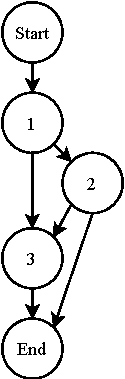
\includegraphics[height=1.5in]{img/Background/control-flow-graph.pdf}
    \label{fig:background_control_flow_graph_image}
    \end{minipage}
&
\begin{minipage}[c]{0.45\textwidth}
\centering
\begin{lstlisting}[language=Python, label=lst:background_control_flow_graph_listing]
def function(a,b):
    if a < b: # (1)
        if b < 10: #(2)
            a = a + b
        else:
            return b #(end)
    a = a * 2 #(3)
    return a #(end)
\end{lstlisting}
\end{minipage}
\end{tabular}
\caption[Control-flow graph visualisation for a code sample]{Control-flow graph visualisation for a code sample. The graph has 6 edges, 5 nodes and one connected component. The cyclomatic complexity is 3. }
\label{fig:background_control_flow_graph}
\end{figure}

The cyclomatic complexity on a control-flow graph as the number of linearly independent execution paths is defined as:
\begin{equation}\label{eq:cyclomatic_complexity}
M = E - N + 2P
\end{equation}

$E$ is the number of edges, $N$ the number of nodes and $P$ the number of connected components.  A connected graph is a subgraph, in which all nodes are connected to each other by a path. Following this definition, the cyclomatic complexity can be calculated. Figure \ref{fig:background_control_flow_graph} shows a visualisation of a sample python function. The control-flow graph has six edges, five nodes and is one connected component. Using equation \ref{eq:cyclomatic_complexity}, the cyclomatic complexity is 3.

MacCabe recommends limiting the cyclomatic complexity to 10. NIST confirms this recommendation in TODO. A lower cyclomatic complexity improves testability since the complexity represents the number of execution paths that need to be tested. Therefore, $M$ is the upper bound for the number of test cases for full branch coverage. 
Furthermore, studies suggest a positive correlation between cyclomatic complexity and defects in functions. TODO source
Software that has to comply to safety standards like ISO 26262 (for electronics in automobiles) or IEC 62304 (for medical devices) are mandated to have a low cyclomatic complexity\cite{isotc_22sc_32_iso_2018, isotisotc_210_iec_2006c_210}.

Although cyclomatic complexity is used throughout the industry, several shortcomings are under critique. First, complexity from data flow is ignored. Working with a larger number of variables and operations, the code becomes more complex, but the cyclomatic complexity does not take this into account. Second, nested code structures are not considered by the metric, although it adds additional difficulty for understanding. TODO source as Halstead critique.

\subsection{Halstead Complexity Measures}
Maurice Halstead introduced the Halstead complexity measures (HCM) in 1977\cite{halstead1977elements}. Halstead approached the complexity measure with an empirical approach by defining observable and measurable properties and put them into relations.

The measurable properties are operators and operands. Operators are symbols in expressions like an addition, subtraction or multiplication symbol. Operands are the values and variables that are manipulated by the operators. 

The sum and number of distinc operators and operands are counted as:
\begin{itemize}
    \item $\eta_1$ as the number of distinct operators 
    \item $\eta_2$ as the number of distinct operands
    \item $N_1$ is the sum of all operators
    \item $N_2$ is the sum of all operands  
\end{itemize}

From these base properties, Halstead derrived additional properties:
\begin{itemize}
    \item Program vocabulary size:
    \begin{displaymath}
        \eta = \eta_1 + \eta_2
    \end{displaymath}
    \item Program length as the sum of all operators and operands:
    \begin{displaymath}
        N = N_1 + N_2
    \end{displaymath}
    \item The volume of a program in terms of program length and program vocabulary is defined as: 
    \begin{displaymath}
        V = N * \log_2{\eta}
    \end{displaymath}
\end{itemize}

Based on those properties, code metrics can be calculated. 
First, the difficulty of understanding a program is calculated as:
\begin{displaymath}
    D = \frac{\eta_1}{2} * \frac{N_2}{\eta2}
\end{displaymath}
The major contributors to difficulty are the number of distinct operators $\eta_1$ and the sum of all operands $N_2$.

Second, the combination of difficulty and volume is the required effort for understanding or changing code follows:
\begin{displaymath}
    E = D * V
\end{displaymath}

Third, the effort for changes translates into real time following the relation:
\begin{displaymath}
    T = \frac{E}{18}s.
\end{displaymath}

Last, the number of bugs correlates with the following relation TODO cite: A survey on metric of software complexity:
\begin{displaymath}
    B = \frac{V}{3000}
\end{displaymath}

HCM focus on the complexity introduced by data manipulation but ignores complexity from the control-flow. Since the cyclomatic complexity focus on the control-flow complexity but not on the data-flow complexity, it is practical to use both together to supplement each drawback (TODO source: A survey on metric of software complexity
). Additionally, the correlation with the number of bugs is based on the programmer's skill estimation with a fixed value of 3000. Since this varies between projects, such an experiential and fixed number is doubtable (TODO source as before).

\subsection{Software Maintainability Index}
The software maintainability index was developed by Dan Coleman and Paul Oman in 1994. 16 HP engineers evaluated 16 software systems and scored it in a range from 0 to 100, with 100 representing best maintainability\cite{coleman_using_1994}. 
Following a regression analysis, they identified the following equation to match the maintainability of the evaluated systems:
\begin{displaymath}
MI = 171 - 5.2 *\ln{\overline{V}} - 0.23 * \overline{M} - 16.2 * \ln{\overline{LOC}} + 50 * \sin{\sqrt{2.4 * C}}
\end{displaymath}
$\overline{V}$ is the average Halstead Volume, $\overline{M}$ the average cyclic complexity, $LOC$ the lines of code and $C$ as fraction of comments.

The software maintainability index was defined many years ago with a limited sample size of developers and projects. Additionally, programming languages have changed significantly over time. A study by Sjøberg et al. suggest no correlation between the software maintainability index and actual maintenance effort in a controlled environment\cite{sjoberg_questioning_nodate}. Although the study only analysis four software projects and lacks generalisation, they find a strong anti-correlation with different maintainability metrics. Only the code size seems to correlate with the actual maintainability. The former seems to be consistent with a systematic review on software maintainability predictions and metrics by Riaz et. al\cite{riaz_systematic_2009}.


\section{Tools for Code Quality Analysis}\label{sec:tool_comparison}
It is good practice to use static code analysis tools to improve code quality. A static code analysis examines a program by analysing an abstract syntax tree, the control or data flow, a pointer analysis or an abstract (approximated) execution. In comparison to dynamic analysis, the code is not executed. The result of static analysis can be based on approximations, so there might be false-positive results. An expert has to examine the result and correct results if necessary\cite{prahofer_static_2017}.

Besides the use of static code analysis for compiler and optimisations, it is also helpful for analysing the code quality. Different categories of code quality-related principles can be analysed:
\begin{description}
    \item[Code Guidelines:] A static code analysis can ensure compliance to structural, naming and formatting code guidelines. 
    \item[Standard Compliance:] A requirement for a software may be compliance to an industry-standard like IEC 61508 or ISO 26262 \cite{noauthor_iec_2010,isotc_22sc_32_iso_2018}. Static code analysis can ensure or at least assist with the compliance.  
    \item[Code Smells:] Some code smells follow a known pattern and a static code analysis can detect those smells. Since code smells can be an indication for chaotic code, it is best if these smells are detected and removed early on.
    \item[Bug Detection:] Although bug detection with static analysis can not detect all bugs, every detected bug before a software release is important. Examples for detected bugs are unhandled expressions or concurrency issues \cite{delaitre_evaluating_2015}.
    \item[Security Vulnerability Detection:] Static code analysis tools can detect some security vulnerabilities like SQL Injection Flaws, buffer overflows and missing input validation with high confidence. Since these are some common, easy to exploit vulnerabilities, an analysis for security vulnerabilities can increase the security of the overall software \cite{wichers_source_nodate}.  
\end{description}

The following sections provide an overview of a few static code analysis tools with a focus on code quality and maintainability. We selected them based on popularity and if the projects are still maintained.

\subsection{PyLint}
PyLint is a code analysis tool for the Python programming language. It is open-source and licensed under the GNU General Public License v2.0 and available for all common platforms. PyLint can be executed as a standalone program or can be integrated into common IDEs like Eclipse. A continuous integration pipeline may include PyLint as well to ensure an analysis on every build.

With PyLint, the developer can make sure the code complies to the PEP8 (TODO) style guide for python coding. This includes name formatting, line length and more. It does not calculate a metric for the code but instead warns about violated principles. Additionally, PyLint can detect common errors like missing import statements that may cause the program to crash at the start or later at runtime. To support refactoring, PyLint can detect duplicated code and will suggest refactoring the code.

PyLint can be configured to ignore some checks and to disable specific rules. To expand the ruleset, a developer can write a "checker", an algorithm to check for a specific rule. The algorithm can analyse the raw file content, a token stream of the source code or an AST representation. The checker can raise a rule violation by providing the location information and the problem type to the PyLint framework and it will be included in the PyLint analysis report.

\subsection{PMD Source Code Analyzer Project}
PMD is an "extensible cross-language static code analyser" for Java, JavaScript and more. As an open-source project, it is licensed under a BSD-style license and is available for macOS, Linux and Windows-based systems. It integrates into build systems like Maven and Gradle as well as into common IDEs like Eclipse and IntelliJ. PMD can run as part of a continuous integration pipeline and is included in the automated code review tool Codacy (see TODO).

Depending on the target language, PMD supports different rules. For Java, PMD has ruled in the following categories:
\begin{description}
    \item[Best practices:] Best practices include rules like one declaration per line or using a logger instead of a \textit{System.out.print()} in production systems.  
    \item[Coding Style and Design] Several rules to improve the readability of the code like naming conventions, ordering of declarations and design problems like a violation of the law of Demeter, Cyclomatic complexity calculation and detection of god classes.
    \item[Multihtreading: ]  Rules to mainly prevent the use of not thread-safe objects or methods. Due to the nature of multi-threading and unpredictable scheduling of threads, problems like unpredictable values of variables or deadlocks may occur. Since they may not occur in every execution, they are hard to spot and to debug. Consequently, warnings of using non-thread-safe code may save hours of debugging.
    \item[Performance: ] These rules flag known operations that have hidden performance implications. For example, string concatenation with the plus operator in Java causes the Java Virtual Machine to create an internal String buffer. This can slow down the program execution if numerous String concatenations are performed.
    \item[Security:] Security-wise, PMD only checks for hardcoded values for cryptographic operations like keys and initialisation vectors.
    \item[Error Prone Code: ] PMD checks for several known code structures that will or may cause a bug at execution. Some rules are part of the clean code principles described in \ref{sec:clean_code} and some rules are specific to the target language.
\end{description}

A user can expand the PMD ruleset in two ways: A XPath expression can be specified and will be validated against the AST by the PMD framework. For more control, it is possible to write a Java-based plugin that implements a custom AST traverser. The latter allows for more sophisticated rules and checks.

\subsection{Codacy}
Codacy is a software to "automate your code quality" (TODO source) for more than 30 programming languages. It is available as a cloud-based subscription service with a free tier for open-source projects and a self-host option for enterprise customers.  Codacy runs as cloud software and a user can connect a GitHub, GitLab or Bitbucket repository that will be scanned automatically on every push or trigger a scan of local files with a command-line program. Additionally, a badge can be added to the readme page to show off the analysis results.

Codacy can be seen as a platform that runs multiple different "analysis engines". These analysis engines combine multiple tools depending on the language. For Python, Codacy uses  PyLint, Bandit (a scanner for security issues) and a metric plugin.
Due to the licensing of those analysis engines, the engines are open-sourced, whereas the Codacy platform is proprietary.

Depending on the language, Codacy supports scanning for common security and maintainability issues. The later is faced with scanning for Code Standardization, Test Coverage and Code Smells to reduce technical debt.

Codacy allows customisation by disabling certain rules and changing rule parameters like the pattern to fit the rules to the project. 

\subsection{Sonarqube}
Sonarqube is an analysis tool to maintain high code quality and security. It supports 15 programming languages in the open-source version licensed under the GNU Lesser General Public License, Version 3.0. In the Developer Edition, Sonarqube supports 22 languages and 27 languages in the enterprise edition. Sonarqube is a self-hostable server application with a SonarScanner client module that can be integrated into build pipelines like Gradle and Maven as well as a command-line tool for other build pipelines. The SonarScanner reports the result to the server, that serves a website to review the results. With the Developer Edition, branch and pull request analysis are possible and a pull request will be annotated with the analysis results.

For Python, Sonarqube offers more than 170 rules. These rules are in the following categories:
\begin{description}
    \item[code Smells:] Code Smells like duplicated String literals are flagged with four different levels of severity (from higher to lower severity): Blocker, Critical, Major, Minor. Explanations and examples are accessible for the developer to understand and fix the issue. The analysis is more in-depth than AST-based solutions since it additionally uses control and data-flow analysis.
    \item[Bug:] Multiple rules cover bugs that would definitively result in a runtime exception and program termination. As an example, calling a function with the wrong number of arguments will be flagged with the highest severity, since it will raise a TypeError during runtime. Although programmers may notice issues like this during coding and testing, the issue can remain hidden if it only triggers a special execution path of the system.
    \item[Security Hotspot: ] The Security Hotspot analysis unfolds pieces of code that may be a real vulnerability and requires a human review. The scanning has a hotspot detection for seven out of the OWASP Top Ten Web Application security risks (TODO src). A flagged hotspot contains a detailed explanation of the reason for being flagged and a guide on how to review this hotspot. The recommendation to double-check a piece of code can help to prevent a security vulnerability from being deployed to production.
    \item[Security Vulnerabilities: ]  A security vulnerabilities analysis reveal code that is at risk of being exploited and has to be fixed immediately. Especially misconfiguration of cryptographic libraries can be revealed easily and future damage prevented.   
\end{description}

Additionally, Sonarqube offers several metrics like test coverage and a custom derivate of Cyclomatic Complexity named Cognitive Complexity\cite{campbell2018cognitive}. The authors see several shortcomings in the original Cyclomatic Complexity model:
\begin{itemize}
    \item Parts of code with the same Cyclomatic Complexity do not necessarily represent an equal difficulty for maintenance.
    \item  Cyclomatic Complexity does not include modern language features like try/catch and lambdas. Therefore, the score can not be accurate.
    \item Cyclomatic Complexity lacks useability on a class or module level. Since the minimum complexity of a method is one and a high aggregated Cyclomatic Complexity for a class is measured for small classes with complex methods or large classes with low complexity per method (e.g. a domain class with just getter/setter).
\end{itemize}
Cognitive Complexity addresses these points, especially the incorporation of modern language features and meaningfulness on class and module level.

The calculation is based on three rules\cite{campbell2018cognitive}:
\begin{description}
    \item[Ignore Shorthand Structures]: Method calls condense multiple statements into one easy to understand the statement. Therefore, method calls as shorthand are ignored for the score. Similarly, shorthand structures like the null-coalescing operator reduce the Cognitive Complexity compared to an extensive null check and are therefore ignored for score calculation.
    \item[Break in the linear control flow]: A break in the expected linear control flow by loop structures and conditionals adds to Cognitive Complexity as to Cyclomatic Complexity. Additionally, Catches, Switches, sequences of logical operators, recursion and jumps also adds to Cognitive Complexity, since these structures break the linear control flow.
    \item[Nested flow-breaking strcutures]: Flow-breaking structures that are nested additionally increase the Cognitive Complexity, since it is harder to understand than non-nested structures.  
\end{description}
The method-level Cognitive Complexity score represents a relative complexity difference between methods that would have the same Cyclomatic Complexity. Furthermore, the aggregated Cognitive Complexity on a class or module level now differentiate between classes with many, simple methods and classes with a few, but complex methods. As a result, domain classes (containing mainly getters/setters) have a lower score compared to classes with complex code behaviour\cite{campbell2018cognitive}.

Developers can extend Sonarqube similarly to PMD. They can write a Java plugin that can access the AST but also a semantic model of the code. Additional, extensions can be created that provide the functionality to other extensions. The Java plugin is compiled into a .jar file and placed into the plugin dir of the Sonarqube installation. For simpler rules, XPath expressions are possible through the web interface and allow a quick extension. For instance, if developers observe bad code style during a pull request review, they can quickly write a rule to enforce this rule in all subsequent pull requests automatically.

Integration in continuous integration, manual review

Tools review for all tools that check different stuff

Single Responsible principle, Open-Closed principle

